%%%%%%%%%%%%%%%%%%%%%%%%%%%%%%%%%%%%%%%%%%%%%%%%%%%%%%%%%%%%%%%%%%%%%%%%%%%%%%%%
% Universität Düsseldorf                                                       %
% Lehrstuhl für Softwaretechnik und Programmiersprachen                        %
% Vorlage für Bachelor- und Masterarbeiten                                     %
% Erstellt: 2019-09-03                                                         %
%%%%%%%%%%%%%%%%%%%%%%%%%%%%%%%%%%%%%%%%%%%%%%%%%%%%%%%%%%%%%%%%%%%%%%%%%%%%%%%%
\documentclass{hhuthesis}


%%%%%%%%%%%%%%%%%%%%%%%%%%%%%%%%%%%%%%%%%%%%%%%%%%%%%%%%%%%%%%%%%%%%%%%%%%%%%%%%
%% Einstellungen zur Personalisierung                                         %%
%%                                                                            %%
%% Im Folgenden können Sie Ihre Arbeit personalisieren.                       %%
%%%%%%%%%%%%%%%%%%%%%%%%%%%%%%%%%%%%%%%%%%%%%%%%%%%%%%%%%%%%%%%%%%%%%%%%%%%%%%%%

%% Spracheinstellung
%% Kommentieren Sie die entsprechende Zeile ein bzw. aus.
%% Wir empfehlen jedem sich an einer englischen Arbeit zu versuchen.
\usepackage[ngerman,english]{babel} % English
%\usepackage[english,ngerman]{babel} % Deutsch

%% Ihr Name
\author{Jan-Eike Brocker}

%% Der Titel der Arbeit
\title{Argument Structure Identification based on Large Language Models}
% \subtitle{Usually not needed}

%% Der zu erreichende Abschluss, entweder Bachelor oder Master
%\graduationtype{Bachelor}
\graduationtype{Master}

%% Ihr Studienfach
\subject{Informatik}

%% Beginn- und Abgabedaten der Arbeit
\begindate{03.~September~2019} % Beginn
\duedate{03.~Dezember~2019} % Abgabe

%% Erst- und Zweitgutachter
\firstexaminer{Prof.~Dr.~Michael~Leuschel}
\secondexaminer{tbd}

%% Farb- oder Schwarzweißdruck
% Benutzen Sie das Kommando \blackwhiteprint,
% wenn sie in schwarzweiß drucken möchten.
% Im Farbdruck ist jede farbige Seite idR teurer.
% \blackwhiteprint % Kommentarzeichen entfernen für Schwarzweißdruck

%%%%%%%%%%%%%%%%%%%%%%%%%%%%%%%%%%%%%%%%%%%%%%%%%%%%%%%%%%%%%%%%%%%%%%%%%%%%%%%%
%% (Ende) Einstellungen zur Personalisierung                                  %%
%%%%%%%%%%%%%%%%%%%%%%%%%%%%%%%%%%%%%%%%%%%%%%%%%%%%%%%%%%%%%%%%%%%%%%%%%%%%%%%%
%% LaTeX Packages in Nutzung                                                  %%
%%                                                                            %%
%% Im folgenden können Sie für die Niederschrift Ihrer Arbeit benötigte       %%
%% LaTeX-Pakete einbinden.                                                    %%
%% Diese Vorlage kommt bereits mit einigen nützlichen inkludierten Paketen.   %%
%%%%%%%%%%%%%%%%%%%%%%%%%%%%%%%%%%%%%%%%%%%%%%%%%%%%%%%%%%%%%%%%%%%%%%%%%%%%%%%%

%% Macht den \todo-Befehl verfügbar.
%% Hiermit können Sie Abschnitte annotieren,
%% welche weiterer Bearbeitung bedürfen.
\usepackage[textsize=scriptsize]{todonotes}

%% Zeige Zeilennummern in der Arbeit an.
%% Der \linenumbers Befehl muss hierzu aufgerufen werden.
%% Praktisch für Feedback Ihrer potentiellen Korrekturleser!
\usepackage{lineno}
% \linenumbers % <- Kommentar entfernen!

\usepackage[T1]{fontenc}
\usepackage{lmodern}

%% Häufig benutzte mathematische Packages.
\usepackage{amsfonts}
\usepackage{amsmath}
\usepackage{amssymb}

\usepackage{siunitx} % \num Befehl zum einfacheren Formatieren von Zahlen.
\usepackage{enumitem} % Leichter konfigurierbare enumerate-Umgebungen.
\usepackage{subcaption} % Unterteilung von Figures in Subfigures.
\usepackage[colorlinks]{hyperref} % Klickbare Links (z.B. Inhaltsverzeichnis).
\sethyperrefpdfinfos{} % Setzt Autor, Titel, etc. als PDF-Metadaten.
\sethyperrefhhucolors{} % Setzt den Farbsatz der HHU für hyperref.
\usepackage{hypcap} % Ankert hyperref links auf Grafik/Tabelle statt Caption.
\usepackage{url} % \url Kommando für Darstellung von Links
\usepackage{csquotes} % Improved quoting.
\usepackage{microtype} % Verbessertes Kerning zwischen Wörtern.

%% Tabellen
\usepackage{tabularx} % tabularx Umgebung für mehr Kontrolle über Tabellen.
\usepackage{booktabs} % \toprule, \midrule, \bottomrule
\usepackage{multirow}
\usepackage{multicol}
\usepackage{longtable} % Große Tabellen gehen über mehrere Seiten.

%% Quellcode
\usepackage{listings} % Einbindung von Code.
\setlstlistingstyle{} % Kosmetische Einstellungen

%% Algorithmen in Pseudocode
\usepackage{algorithm} % Float-Umgebung für angegebene Algorithmen.
\usepackage{algorithmicx} % Angabe von Algorithmen in Pseudocode.
\usepackage{algpseudocode} % Standard Pseudocode-Elemente für Algorithmen.
\setalgorithmstyle{} % Kosmetische Einstellungen

%% Intelligenteres Referenzieren mittels \cref.
%% \languagename um dynamisch zwischen ngerman oder english zu wechseln.
\usepackage[\languagename,capitalize,noabbrev]{cleveref}

%%%%%%%%%%%%%%%%%%%%%%%%%%%%%%%%%%%%%%%%%%%%%%%%%%%%%%%%%%%%%%%%%%%%%%%%%%%%%%%%
%% (Ende) LaTeX Packages in Nutzung                                           %%
%%%%%%%%%%%%%%%%%%%%%%%%%%%%%%%%%%%%%%%%%%%%%%%%%%%%%%%%%%%%%%%%%%%%%%%%%%%%%%%%


\begin{document}
%% Set up title page, declaration of authorship, abstract, acknowledgements
\frontmatter
\makefrontmatter

%%%%%%%%%%%%%%%%%%%%%%%%%%%%%%%%%%%%%%%%%%%%%%%%%%%%%%%%%%%%%%%%%%%%%%%%%%%%%%%%
%% Danksagungen                                                               %%
%%%%%%%%%%%%%%%%%%%%%%%%%%%%%%%%%%%%%%%%%%%%%%%%%%%%%%%%%%%%%%%%%%%%%%%%%%%%%%%%
\begin{acknowledgements}
  Im Falle, dass Sie Ihrer Arbeit eine Danksagung für Ihre Unterstützer
  (Familie, Freunde, Betreuer)
  hinzufügen möchten, können Sie diese hier platzieren.

  Dieser Part ist optional und kann im Quelltext auskommentiert werden.
\end{acknowledgements}
%%%%%%%%%%%%%%%%%%%%%%%%%%%%%%%%%%%%%%%%%%%%%%%%%%%%%%%%%%%%%%%%%%%%%%%%%%%%%%%%
%% (Ende) Danksagungen                                                        %%
%%%%%%%%%%%%%%%%%%%%%%%%%%%%%%%%%%%%%%%%%%%%%%%%%%%%%%%%%%%%%%%%%%%%%%%%%%%%%%%%


\tableofcontents


\mainmatter

%%%%%%%%%%%%%%%%%%%%%%%%%%%%%%%%%%%%%%%%%%%%%%%%%%%%%%%%%%%%%%%%%%%%%%%%%%%%%%%%
%% Der Inhalt der Arbeit                                                      %%
%%                                                                            %%
%% Hier können Sie die schriftliche Ausarbeitung ihrer Arbeit                 %%
%% niederschreiben. Der Übersicht halber bietet sich jedoch an, dies in einer %%
%% oder mehreren separaten Dateien zu tun, welche mittels \input eingebunden  %%
%% werden --- wie auch in der Vorlage geschieht.                              %%
%%%%%%%%%%%%%%%%%%%%%%%%%%%%%%%%%%%%%%%%%%%%%%%%%%%%%%%%%%%%%%%%%%%%%%%%%%%%%%%%

%%%%%%%%%%%%%%%%%%%%%%%%%%%%%%%%%%%%%%%%%%%%%%%%%%%%%%%%%%%%%%%%%%%%%%%%%%%%%%%%%%
% Diese Datei beinhaltet den eigentlichen Inhalt Ihrer Arbeit.
%
% Es bietet sich der Übersicht halber an, die einzelnen Abschnitte jeweils
% in eigene Dateien zu schreiben und mittels \input einzubinden.
% Eine mögliche Verzeichnisstruktur sähe entsprechend so aus:
%
%     thesis/
%     +- tex/
%     |  +- introduction.tex
%     |  +- motivation.tex
%     |  +- experiments.tex
%     |  |  ...
%     |  +- conclusion.tex
%     +- abstract.tex
%     +- contents.tex
%     +- thesis.tex
%%%%%%%%%%%%%%%%%%%%%%%%%%%%%%%%%%%%%%%%%%%%%%%%%%%%%%%%%%%%%%%%%%%%%%%%%%%%%%%%

\section{Einleitung}

Dies ist der Hauptteil Ihrer Arbeit.
Hier leiten Sie grob in das Thema ein, motivieren es und geben einen Ausblick
über das, was Sie in Ihrer Arbeit behandeln werden.

Der Inhalt der Vorlage ist mit Beispielen gefüllt, wie man \LaTeX{}
verwendet und traditionelle Stolpersteine vermeidet.
Lesen Sie die Vorlage gründlich.


\subsection{Makefile}

Im Wurzelverzeichnis finden Sie ein \texttt{Makefile}.
Über das Terminal können Sie die folgenden Befehle aufrufen,
wie in \cref{tab:make} beschrieben.


\begin{table}[h]
  \centering
  \caption{Übersicht der \texttt{Makefile}-Befehle.}%
  \label{tab:make}
  \begin{tabularx}{\textwidth}{lX}
    \toprule
    Befehl & Effekt \\
    \midrule
    \texttt{make} & Kompiliert das PDF und löscht aux-Files. \\
    \texttt{make clean} & Löscht das PDF und dazugehörige aux-Files. \\
    \texttt{make bibtool} & Sortiert \texttt{references.bib}
    und formatiert die Einträge einheitlich. \\
    \texttt{make watch} & Rekompiliert das PDF bei Änderungen und
    hält die Anzeige in Ihrem PDF-Betrachter aktuell. \\
    \bottomrule
  \end{tabularx}
\end{table}


\section{Referenzen und Zitationen}

In der Datei \texttt{references.bib} finden Sie bereits einige Quellen,
die Sie wahrscheinlich zitieren mögen,
wie z.B. die B Methode~\cite{abrial1996b,abrial2010modeling}
oder \textsc{ProB}~\cite{leuschel2003prob,leuschel2008prob}.
Beachten Sie den Artikel ``Common Errors in Bibliographies'' von John Owens.%
\footnote{\url{https://www.ece.ucdavis.edu/~jowens/biberrors.html}}
Zusätzliche, ausführlichere Informationen finden Sie auch in \cref{app:sec:bib}.


\subsection{Referenzen platzieren}

Sie platzieren Referenzen mit \texttt{\textbackslash{}cite{}}.
Diese sollten jeweils hinter dem Namen der zitierten Technik stehen,
oder hinter der zu belegenden Aussage.
Im Falle, dass sich ein gesamter Absatz auf eine einzelne Quelle bezieht,
genügt es die Referenz im ersten Satz anzugeben, solange vom Kontext klar ist,
dass der restliche Absatz sich ebenfalls auf die Quelle bezieht.
Referenzen sind nicht erst am Ende eines gesamten Absatzes zu platzieren.
Ebenso sind sie Teil des Satzes und stehen vor dem abschließenden Punkt.

\begin{itemize}
  \item Gut: \enquote{\textsc{ProB}~\cite{leuschel2003prob} is an
    animator, model checker, and constraint solver for the B method~\cite{abrial1996b}.
    The B method allows to specify, design, and code
    software systems as well as to perform formal proof of their properties.}
  \item Nicht gut: \enquote{\textsc{ProB} is an
    animator, model checker, and constraint solver for the B method~\cite{leuschel2003prob,abrial1996b}.
    The B method allows to specify, design, and code
    software systems as well as to perform formal proof of their properties.}
  \item Nicht gut: \enquote{\textsc{ProB} is an
    animator, model checker, and constraint solver for the B method
    The B method allows to specify, design, and code
    software systems as well as to perform formal proof of their properties.~\cite{leuschel2003prob,abrial1996b}}
\end{itemize}


\subsection{Über Literatur sprechen}

Obwohl die Referenzen innerhalb des Satzes stehen, sind sie keine Wörter.
Sie ersetzen somit nicht die explizite Nennung einer Quelle.
Sollte über ein bestimmtes Papier gesprochen werden, so ist dieses via
Autorennamen zu betiteln. Hierbei gilt:
\begin{itemize}
  \item Es sind nur die Nachnamen zu verwenden,
  \item hinter den Autorennamen ist die Referenz zu setzen,
    falls der Bezug unklar ist,
  \item ab drei oder mehr Autoren wird nur der Erstautor geführt, gefolgt von
    \enquote{et al.}.
\end{itemize}

So schreiben wir
\enquote{SICStus Prolog~\cite{carlsson1988sicstus} wurde von Carlson et al.\
  entwickelt}
oder
\enquote{Leuschel \& Butler~\cite{leuschel2003prob} haben einen Model Checker für die
  B-Methode~\cite{abrial1996b} entwickelt}.
Falsch hingegen ist es, eine Referenz als eigenständiges Wort zu nutzen, wie in
folgendem Negativbeispiel:
\enquote{In \cite{leuschel2003prob} wurde ein Model Checker für die B-Methode entwickelt}.



\section{Bilder und Tabellen}

Bilder und Tabellen sind per se wie von \LaTeX{} bekannt zu setzen.
Wichtig ist, dass sie ausnahmslos im Fließtext referenziert wurden.
Eine nichtreferenzierte Tabelle oder Abbildung kann ebenso ausgelassen werden.
Solche Querverweise werden in \cref{sec:references} besprochen.


\subsection{Bilder}%
\label{sec:figures}

\Cref{fig:initial-draft} ist eine exemplarische Abbildung, auf die an dieser
Stelle im Text verwiesen wird.
Stilistisch ist es meist empfehlenswert innerhalb der
\texttt{figure}-Umgebung ein \texttt{\textbackslash{}centering} zu setzen,
sodass der Inhalt zentriert wird.
In \cref{fig:hhu-logo} wird ein Beispiel der
\texttt{\textbackslash{}subfigure}-Umgebung aus dem
\texttt{\textbackslash{}subcaption}-Paket demonstriert.
Beide Teilabbildungen, \cref{fig:hhu-rgb,fig:hhu-bw},
sind individuell referenzierbar.

\begin{figure}[h]
  \centering
  
\includegraphics[width=4cm]{fig/the.png}
  \caption{Initial thesis draft.}%
  \label{fig:initial-draft}
\end{figure}

\begin{figure}[h]
  \begin{subfigure}{.5\textwidth}
    \centering
    
\includegraphics[width=4cm]{fig/hhu-logo-rgb.pdf}
    \subcaption{in Farbe}%
    \label{fig:hhu-rgb}
  \end{subfigure}% <- Kommentarzeichen am Ende der Zeile ist wichtig!
  \begin{subfigure}{.5\textwidth}
    \centering
    
\includegraphics[width=4cm]{fig/hhu-logo-black.pdf}
    \subcaption{Schwarzweiß}%
    \label{fig:hhu-bw}
  \end{subfigure}% <- Kommentarzeichen am Ende der Zeile ist wichtig!
  \caption{Das neue HHU-Logo.}%
  \label{fig:hhu-logo}
\end{figure}


\subsection{Tabellen}%
\label{sec:tables}

Während bei Abbildungen die \texttt{\textbackslash{}caption}
in aller Regel unter dem Bild steht,
wird sie bei Tabellen typischer Weise darüber platziert, wie bei
\cref{table:truths} zu sehen.

\begin{table}[ht]
  \begin{center}
    \caption{Table of truths.}%
    \label{table:truths}
    \begin{tabular}{lr}
      \toprule
      Fakt                                & Wahrheitsgehalt \\
      \midrule
      booktabs-Tabellen sind hübscher     & 90 \%           \\
      Han Solo schoss zuerst              & 100 \%          \\
      Game of Thrones fand ein gutes Ende & 0 \%            \\
      \bottomrule
    \end{tabular}
  \end{center}
\end{table}

Es ist zu empfehlen, das Paket \texttt{booktabs} zur Formatierung der Tabellen
zu nutzen.
Dieses empfiehlt die Verwendung der Befehle
\texttt{\textbackslash{}toprule},
\texttt{\textbackslash{}midrule} und
\texttt{\textbackslash{}bottomrule},
und rät davon ab, vertikale Linien zu nutzen.
Vergleichen Sie \cref{tab:booktabs-yes,tab:booktabs-yesnt}.

\begin{table}
  \centering
  \caption{Vergleich von \LaTeX{}-Tabellen mit und ohne booktabs.}
  \begin{subtable}{.5\textwidth}
    \centering
    \subcaption{mit booktabs}%
    \label{tab:booktabs-yes}
    \begin{tabular}{lrr}
      \toprule
      Backend & Accuracy & F\textsubscript{1}-Score \\
      \midrule
      CLP(FD) & 0.947 & 0.966 \\
      Z3      & 0.919 & 0.797 \\
      \bottomrule
    \end{tabular}
  \end{subtable}%
  \begin{subtable}{.5\textwidth}
    \centering
    \subcaption{ohne booktabs}%
    \label{tab:booktabs-yesnt}
    \begin{tabular}{|l|r|r|}
      \hline
      Backend & Accuracy & F\textsubscript{1}-Score \\ \hline
      CLP(FD) & 0.947 & 0.966 \\ \hline
      Z3      & 0.919 & 0.797 \\ \hline
    \end{tabular}
  \end{subtable}%
\end{table}



\subsection{Plots}%
\label{sec:plot}

Sie können mithilfe von \texttt{tikz} und \texttt{pgfplots}
Graphen oder Bar Charts erstellen,
wie in \cref{fig:the-plot,fig:long-caption} der gezeigt ist.
Beachten Sie, dass die Vorlage die Cycle Lists
\texttt{hhubwcycle} (schwarzweiß) und \texttt{hhucolorcycle} bereit stellt,
welche die offiziellen HHU-Farben zur Darstellung der verschiedenen Graphen
verwendet.
Diese können in jeglichem \texttt{tikzplot} mittels der Option
\texttt{cycle list name=} gesetzt werden und stehen, je nach Druckeinstellung
innerhalb der PDF via \texttt{\textbackslash{}blackwhiteprint}
entweder automatisch auf \texttt{hhucolorcycle} oder \texttt{hhubwcycle}.

\begin{figure}[ht]
  \centering
  \begin{subfigure}{.5\textwidth}
    \centering
    \begin{tikzpicture}
      \begin{axis}[
        width=\textwidth,
        cycle list name=hhucolorcycle
      ]
        \foreach \y in {0,0.1,...,1} % Wiederholt \addplot mit jeweils anderem \y
          \addplot coordinates {
              ( 1, 3.0 -\y)
              ( 2, 3.25-\y)
              ( 3, 3.5 -\y)
              ( 4, 3.75-\y)
              ( 5, 4.0 -\y)
            };
      \end{axis}
    \end{tikzpicture}
    \subcaption{in den HHU-Farben}
  \end{subfigure}%
  \begin{subfigure}{.5\textwidth}
    \centering
    \begin{tikzpicture}
      \begin{axis}[
        width=\textwidth,
        cycle list name=hhubwcycle % <- Änderung auf schwarzweiß.
      ]
        \foreach \y in {0,0.1,...,1} % Wiederholt \addplot mit jeweils anderem \y
          \addplot coordinates {
              ( 1, 3.0 -\y)
              ( 2, 3.25-\y)
              ( 3, 3.5 -\y)
              ( 4, 3.75-\y)
              ( 5, 4.0 -\y)
            };
      \end{axis}
    \end{tikzpicture}
    \subcaption{in schwarzweiß}
  \end{subfigure}%
  \caption{A beautiful plot.}%
  \label{fig:the-plot}
\end{figure}

\begin{figure}[ht]
  \centering
  \begin{tikzpicture}
    \begin{axis}
      [
        ybar,
        xtick=data,
        enlarge x limits=1,
        symbolic x coords={A, B},
        ymin=0, ymax=100,
        ylabel={$\%$ percentage of bar height},
      ]
      \addplot coordinates {(A,90) (B, 90)};
      \addplot coordinates {(A,75) (B, 75)};
      \addplot coordinates {(A,60) (B, 60)};
      \addplot coordinates {(A,45) (B, 45)};
      \addplot coordinates {(A,30) (B, 30)};
      \legend{blue, red, green, orange, cyan}
    \end{axis}
  \end{tikzpicture}
  \caption[Bar plot with short version of caption for List of Figures]{%
    A really long caption title. This demonstrates how to describe stuff seen
    in the figure, like here, where we see a bar plot showing my favourite
    pies. Nah, actually it shows something completely different.
  }\label{fig:long-caption}
\end{figure}



\section{Querverweise}\label{sec:references}

Für Querverweise, wie zu
\cref{fig:initial-draft,fig:hhu-logo,fig:the-plot,fig:long-caption},
\cref{lst:hello-c,lst:hello-prolog}
oder \cref{alg:minimax}
stehen zwei Möglichkeiten zur Verfügung:
die \LaTeX{}-Standardvariante via \texttt{\textbackslash{}ref},
oder (eleganter) das \texttt{cleveref}-Paket.

Cleveref ermittelt automatisch, welche Art von Element referenziert wird
und fügt den entsprechenden Titel hinzu. Entsprechend sind die in
\cref{tab:cleveref} aufgeführten Beispiele äquivalent.

\begin{table}[ht]
  \centering
  \caption{Vergleich \texttt{\textbackslash{}reg} und \texttt{\textbackslash{}cref}.}%
  \label{tab:cleveref}
  \begin{tabularx}{\textwidth}{XX}
    \toprule
    \LaTeX{} & Darstellung \\
    \midrule
    \lstinline[language=tex]|Abbildung \\ref\{fig:logo\} zeigt das Logo.| &
      Abbildung \ref{fig:hhu-logo} zeigt das Logo. \\
    \lstinline[language=tex]|\\cref\{fig:logo\} zeigt das Logo.| &
      \cref{fig:hhu-logo} zeigt das Logo. \\
    \midrule
    \lstinline[language=tex]|Abbildungen \\ref\{fig:plot1\} und|
      \lstinline[language=tex]|\\ref\{plot2\} sind Graphen.| &
    Abbildungen \ref{fig:the-plot} und \ref{fig:long-caption} sind Graphen.\\
    \lstinline[language=tex]|\\Cref\{fig:plot1,plot2\} sind Graphen.| &
    \Cref{fig:the-plot,fig:long-caption} sind Graphen.\\
    \bottomrule
  \end{tabularx}
\end{table}



\section{Formeln}

\Cref{eq:example1} gibt eine referenzierbare Formel an,
während \cref{eq:example2} eine Formel darstellt, die länger ist, als die
Zeile zulässt.

\begin{equation}
  \label{eq:example1}
  2 = 1 + 1
\end{equation}

\begin{multline}
  \label{eq:example2}
  30 = 1 + 1 + 1 + 1 + 1 + 1 + 1 + 1 + 1 + 1 + 1 + 1 + 1 + 1 + 1 + 1 + 1 + 1 \\
      + 1 + 1 + 1 + 1 + 1 + 1 + 1 + 1 + 1 + 1 + 1 + 1
\end{multline}

In der zweizeiligen Gleichung
\begin{equation}
  \label{eq:mlp-stacking}
  \begin{split}
    \hat{y} & = f_2(f_1(x; W); V) \\
            & = f(x; W, V)
  \end{split}
\end{equation}
wurden die Gleichheitszeichen in beiden Zeilen direkt untereinander ausgerichtet
(mittels \texttt{\&} im Quelltext und der \texttt{split}-Umgebung).
Teilen wir \cref{eq:mlp-stacking}, welche den Forward Pass eines Neuronalen
Netzes darstellt,
in mehrere Schritte auf, so erhalten wir (mittels \texttt{align}-Umgebung)
\begin{align}
  a       & = W^\mathsf{T} x \label{eq:fp-act} \\
  h       & = g_1(a) \label{eq:fp-hidden} \\
  o       & = V^\mathsf{T} h \label{eq:fp-out} \\
  \hat{y} & = g_2(o) \label{eq:fp-pred}
  \,\text{,}
\end{align}
wobei \cref{eq:fp-act,eq:fp-hidden,eq:fp-out,eq:fp-pred} jeweils eine eigene
Referenznummer erhalten.


\section{Algorithmen}

Für Algorithmen kann das bereits inkludierte Paket \texttt{algorithmicx}
genutzt werden.
In \cref{alg:minimax} wird exemplarisch eine Implementierung des
Minimax-Algorithmus aufgeführt.
Beachten Sie, dass \cref{line:commented} kommentiert und referenzierbar ist.

\begin{algorithm}
  \caption{Determining the next action by Minimax}%
  \label{alg:minimax}
  \begin{algorithmic}[1]
    \Function{Minimax}{Game State Tree: $G^n$}
      \State bestValue \(\gets -\infty\)
      \State \(\mathit{bestAction} \gets \) NIL
      \ForAll{\(G^n_a \in S(G^n)\)}
        \State \(\mathit{value} = \) \Call{MinimaxValue}{\(G^n_a\), true}
        \If{\(\mathit{value} > \mathit{bestValue}\)}
          \Comment{Aktualisiere besten Wert}\label{line:commented}
          \State \(\mathit{bestValue} \gets \mathit{value}\)
          \State \(\mathit{bestAction} \gets a\)
        \EndIf
      \EndFor
      \State \Return \(\mathit{bestAction}\)
    \EndFunction
    \Statex
    \Function{MinimaxValue}{Game State Tree: $G^n$, Boolean: $\mathit{ourTurn}$}
      \If{\(D(G^n)=0\)}
        \State \Return \Call{Heuristic}{root(\(G^n\))}
      \ElsIf{\(\mathit{ourTurn}\)}
        \State \(\mathit{maxValue} \gets -\infty \)
        \ForAll{\(S \in S(G^n)\)}
          \State \(\mathit{newValue} \gets \) \Call{MinimaxValue}{\(S\), false}
          \State \(\mathit{maxValue} \gets
            \max(\mathit{newValue}, \mathit{maxValue})\)
        \EndFor
        \State \Return \(maxValue\)
      \Else
        \State \(minValue \gets +\infty \)
        \ForAll{\(S \in S(G^n)\)}
          \State \(\mathit{newValue} \gets \) \Call{MinimaxValue}{\(S\), true}
          \State \(\mathit{minValue} \gets
            \min(\mathit{newValue}, \mathit{minValue})\)
        \EndFor
        \State \Return \(minValue\)
      \EndIf
    \EndFunction
  \end{algorithmic}
\end{algorithm}


\section{Source Code Listings}

\Cref{lst:hello-c,lst:hello-python} zeigen ein `Hello World'-Programm,
je in C und Python.
\Cref{lst:hello-prolog} zeigt ein Prolog-Prädikat, welches eine Liste in zwei
Teile teilen kann.

\begin{lstlisting}[
  float, caption={Hello World in C.}, label={lst:hello-c}, language=C
]
#include <stdio.h>

int main(int argc, char[] *args){
  printf("Hello World!\n");
  // And done!
}
\end{lstlisting}

\begin{lstlisting}[
  float, caption={Totally minimal Hello World in Python.},
  label={lst:hello-python}, language=Python
]
def hello_world():
  print("Hello World"!)

if __name__ == "__main__":
  hello_world()
\end{lstlisting}

\begin{lstlisting}[
  float, caption={Prolog implementation of \texttt{split/4}},
  label={lst:hello-prolog}, language=Prolog
]
% Split list into two parts (length of first list given).
%
% ?- split([a,b,c,d,e,f,g,h,i,k], 3, L1, L2).
% L1 = [a,b,c]
% L2 = [d,e,f,g,h,i,k]
%
split(L, N, L1, L2) :-
  length(L1, N),
  append(L1, L2, L).
\end{lstlisting}


\section{Todonotes}

Es bietet sich an, während der Verschriftlichung Gebrauch von dem
\texttt{todonotes}-Package zu machen.\todo[]{Lernen, wie man mit todonotes umgeht.}

Abgesehen davon, dass es erlaubt die PDF mit offenen Todos zu annotieren,
sind sie ein guter Weg um potentziellen Korrekturlesern zu kommunizieren,
welche Teile ohnehin noch nicht ausgearbeitet sind.
Des Weiteren lässt sich mit
\texttt{\textbackslash{}listoftodos} eine Übersicht der noch offenen Todos
im Dokument anzeigen

\listoftodos

\todo[inline]{Lerne was man machen kann, wenn man einzeln stehende Todos braucht.}
\todo[inline]{Lerne ebenfalls, \texttt{\textbackslash missingfigure} zu nutzen.}
\todo[inline]{Verschaffung eines Überblicks der in der Vorlage inkludierten Pakete.}


\subsection{Missingfigure}

Mittels \texttt{\textbackslash{}missingfigure} lassen sich bereits Abbildungen
im PDF darstellen, die noch erstellt werden müssen. Dies ermöglicht bereits einen
ersten Eindruck, wie das Layout um die Abbildung herum aussehen wird,
wie \cref{fig:missing} exemplarisch zeigt.

\begin{figure}
  \centering
  \missingfigure{Plot is still to be done, but the results from the HPC are not
    yet available.}
  \caption{Finale Laufzeiten meiner unfassbar guten Auswertung.}%
  \label{fig:missing}
\end{figure}


\section{Häufige Fehler}

Der wohl häufigste Fehler, den neue \LaTeX-Nutzer machen, ist eine falsche
Verwendung von Anführungszeichen.
Um dem Vorzubeugen sowie konsistente Anführungszeichen zu nutzen,
empfehlen wir den Einsatz von \texttt{\textbackslash{}enquote}
aus dem bereits inkludierten \texttt{csquotes}-Pakt.
% Dieses erlaubt ebenfalls eine gezielte und automatische Unterscheidung
% zwischen den \foreignquote{english}{englischen} und
% \foreignquote{german}{deutschen} Anführungszeichen.
Wird hingegen, wie in der Programmierung üblich, \textquotedbl verwendet,
versucht \LaTeX{} daraus einen Umlaut zu erzeugen.
So wird beispielsweise \texttt{\textquotedbl{}a} zu ä.

\Cref{tab:quotes} gibt eine Übersicht über verschiedene Möglichkeiten
Anführungszeichen zu setzen und demonstriert die falsche Verwendung von
\textquotedbl.

\begin{table}[ht]
  \centering
  \caption{Demonstration von csquotes.}%
  \label{tab:quotes}
  \begin{tabularx}{\textwidth}{XX}
    \toprule
    \LaTeX{} & Darstellung \\
    \midrule
    \texttt{Ein \textquotedbl{}Wort\textquotedbl{} in \textquotedbl{}Anführungszeichen\textquotedbl{}} &
      Ein "Wort" in "Anführungszeichen" \\ \addlinespace
    \texttt{Ein \textbackslash{}glqq Wort
        in \textbackslash{}glq Anführungszeichen\textbackslash{}grq\textbackslash{}grqq}&
      Ein \glqq Wort in \glq Anführungszeichen\grq\grqq \\ \addlinespace
    \texttt{Ein \textbackslash{}enquote\{Wort
        in \textbackslash{}enquote\{Anführungszeichen\}}\} &
      Ein \enquote{Wort in \enquote{Anführungszeichen}} \\
    \bottomrule
  \end{tabularx}
\end{table}

\section{Conclusion}

Am Ende der Arbeit werden noch einmal die erreichten Ergebnisse
zusammengefasst und diskutiert.


\section{Introduction}
\subsection{Motivation}
Often times in natural language, one uses certain phrases to connect sentences, especially in a discourse setting. These phrases, called discourse markers, are used to connect parts of a text or conversation \cite{Discours1999}. They are also called linking words, which is the term we are going to use over the course of this thesis. Examples of these linking words are \say{therefore}, \say{because}, \say{yet}, \say{in conclusion}, and \say{however}. The word \say{therefore} can, for example, indicate a reasoning while the phrase \say{in conclusion} indicates a conclusion. \\
In this thesis, we want to investigate whether or not linking words can help improve classifiers to identify argument structures in the English language by creating additional features based on probabilities for these linking words to be at a certain position in a text. We will determine these probabilities using masked language models.
\subsection{Tasks}
We are using two classification tasks to evaluate the performance of our approach, namely argument validity prediction and argument stance detection. The former describes the problem of determining whether a conclusion for a given text is valid. The latter is the problem of determining whether a given argument is for or against a certain topic. \\


\section{Theoretical background and related work} \label{theory}
In this chapter, we will explain all the relevant background information needed to follow along with the thesis. \\
We will start by defining the main tasks and continue with describing all the used machine learning techniques. The last section will be about metrics for evaluation.

\subsection{Tasks}
We are going to evaluate our approaches on the two following tasks.

\subsubsection{Validity Classification}
As described in \cite{argsvalidnovel2022}, a conclusion of a premise is considered valid if it follows naturally from its premise. In our case, a premise is a statement consisting of at least one sentence regarding a certain topic and a conclusion consists of exactly one sentence that sums up the premise.\\
Following this definition, validity classification is a binary classification task in which we want to determine whether a conclusion is valid, given its premise. The label $1$ corresponds to a valid conclusion and the label $0$ to an invalid conclusion \cite{argsvalidnovel2022}. An example is shown in figure \ref{fig:val_class1}.

\begin{figure}[H]
  \begin{center}
   	\begin{tabular}{|| c | c | c||}
   	\hline
   	Premise & Conclusion & Validity \\ [0.5ex]
   	\hline\hline
   	\multirow{2}{*}{\makecell{A November 2009 CBS News Poll found \\ that only 40 percent of Americans \\ want Mohammed and his four minions \\ to be tried in federal criminal court.}} & Wind energy is free. & 0 \\\cline{2-3}
 	& \makecell{Majority of Americans \\ are opposed to civilian \\ trial of terrorists.} & 1 \\
 	\hline
	\end{tabular}
  \end{center}
  \caption{Example for validity classification.}%
  \label{fig:val_class1}
\end{figure}

Since we are only interested in the validity of the conclusion, comparisons to the Validity and Novelty Prediction Shared Task \cite{argsvalidnovel2022}, from which we adapted the task, are less meaningful because they classify validity and another label called novelty at the same time. Hence we will adapt their baseline for our task and use this to compare our models.


\subsubsection{Stance Detection}

Our second main tasks is called stance detection. It is a classification task in which we want to decide whether an argument which consists of at least one sentence, is for (positive stance) or against (negative stance) a certain statement which consists of one sentence about some topic \cite{mohammad2017stance}. A positive stance towards the statement corresponds to the label $1$ and a negative stance corresponds to the label $0$. Stance detection can be extended to have a third label which corresponds to a neutral opinion towards the statement but we will stick with the binary version in this thesis. An example for stance detection is shown in figure \ref{fig:stance_class1}.

\begin{figure}[H]
  \begin{center}
   	\begin{tabular}{|| c | c | c||}
   	\hline
   	Statement & Argument & Stance \\ [0.5ex]
   	\hline\hline
   	\multirow{2}{*}{\makecell{ We should limit \\ executive \\ compensation.}} & \makecell{A company can pay higher to their \\ employees if executive compensation is limited.} & 1 \\\cline{2-3}
 	& \makecell{A company has the right to determine how \\ much executive compensation they can pay out.} & 0 \\
 	\hline
	\end{tabular}
  \end{center}
  \caption{Example for stance detection.}%
  \label{fig:stance_class1}
\end{figure}

\subsection{Linking words}
As described in the beginning, we will use the probabilities of linking words to be at a certain position in a text to create additional features for our classifiers. We will use different lists of linking words as well as a list of words which are not necessarily considered linking words. The main list of linking words is the following:

\begin{center}
	[because, although, therefore, but, still, whereas, while, however, since, therefore, as, for, consequently, hence, thus, so, nevertheless, yet, anyway, still, and]
\end{center}

The other lists can be found in the appendix.

\subsection{Language Models}
As hinted in the introduction, we will use language models to assign probabilities to linking words at certain positions in a text. A language model (LM) is a model that assigns probabilities to sequences of words \cite{languagemodels2023}. There are various types of LMs, achieving better performances in different areas. Especially since the release of ChatGPT \cite{chatgpt}, autoregressive models like GPT-3 have become very popular. These models assign probabilities to words, based on the context before the word and therefore generate one word after another based on these probabilities to generate text \cite{gpt3}. Other models, like BERT \cite{bert}, use a bidirectional approach which we will explain in detail in the next part. These bidirectional models are able to predict a masked word from a sentence, based on its left and right context. The model will then return a set of words and their corresponding probabilities to fill this [MASK] token \cite{bert}, as shown in figure \ref{fig:bert_masking_example}.

\begin{figure}[H]
  \begin{center}
	\textit{Berlin is the capital of} \textbf{[MASK]}.
  \end{center}
  \centering
  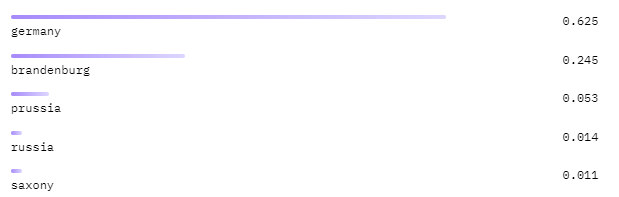
\includegraphics[scale=0.9]{fig/bert_masking_example.png}
  \caption{Example for masking of language models \cite{bertbaseuncased}, accessed 20-October-2023. The figure shows the 5 most likely words and their corresponding probabilities for the [MASK] token in the sentence above.}%
  \label{fig:bert_masking_example}
\end{figure}

We will present another example (see figure \ref{fig:bert_masking_example2}), showing the capability of language models to also predict linking words since this will be the main focus of this work.

\begin{figure}[H]
  \begin{center}
	\textit{Pizza tastes good}, [MASK] \textit{it's one of the most liked foods in the world}.
  \end{center}
  \centering
  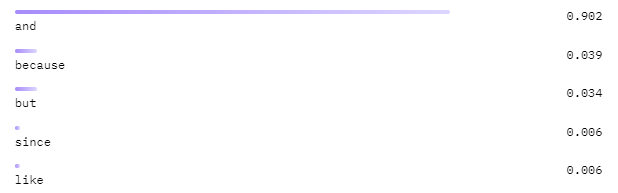
\includegraphics[scale=0.9]{fig/bert_masking_example2.png}
  \caption{Example for linking word masking of language models \cite{bertbaseuncased}, accessed 20-October-2023. The figure shows the 5 most likely words and their corresponding probabilities for the [MASK] token in the sentence above.}%
  \label{fig:bert_masking_example2}
\end{figure}

The second example shows why we need to use bidirectional models instead of autoregressive models like GPT-3 since the linking word is dependent of both its left and right context. \\
LMs are often times pre-trained on large unlabeled text corpora to generate language representations like word vector embeddings which can later be fine-tuned on more specific tasks. In the next sections, we will present two models that we are going to use.


\subsubsection{BERT}
BERT (Bidirectional Encoder Representations from Transformers) is a LM proposed by Devlin et al. \cite{bert}. Unlike older language models based on LSTMs which can only predict the next token based on the previous tokens, BERT uses a bidirectional approach. This is done by using the aforementioned masked LM pre-training objective. In this approach, a part of the input words gets masked and the training objective is to predict the original word based on its left and right context. Together with the next sentence prediction objective, this completes the pre-training for BERT. This model can now be used to solve many downstream tasks like classification or question answering, just by adding another layer on top, depending on the specific task. BERT set new state-of-the-art performances for many NLP tasks and revolutionized the classic NLP pipeline due to it representing all the steps of the pipeline in one model \cite{bertexplain}.  \\
We will primarily use BERT for masked language modeling and directly for validity and stance classification. There are different types of BERT one can consider, differing for example in the number of parameters, language or case sensitivity. The exact configurations and models used, will be explained in detail in the chapter about implementation. \\

\textbf{Model Architecture} \\
Although we do not need to understand BERT in every detail, one important part is needed in the course of this thesis, namely how the input and output is represented. \\
Most importantly, for every input sequence, a special [CLS] token will be added as first character. This token is used in the last hidden state as an aggregate representation for the entire sequence. It can then be used for further downstream tasks like classification. The vector representations for all the other tokens in the output sequence are only used for token-level tasks like part-of-speech-tagging. Furthermore, a [SEP] token is added after each input sequence. With this technique, we can input two sequences as one into BERT which is used to perform the next sentence prediction task in the pre-training \cite{bert}.


\subsubsection{RoBERTa}
RoBERTa is a LLM based on BERT \cite{roberta}. It improves BERT by
\begin{enumerate}
	\item longer training with more data,
	\item removing the next sentence prediction objective,
	\item training on longer sequences,
	\item dynamically changing the masking pattern.
\end{enumerate}
We are going to use RoBERTa as well since it is commonly used in the approaches described in \cite{argsvalidnovel2022}.

\subsection{Gradient-Boosted Trees}
To classify embeddings which will be created by our linking word probabilities, we are going to primarily use two different ways. The first one is a simple neural network as it is used as additional layer for BERT in a classification setting. The other one will be a Gradient-Boosted Tree. Besides its competitive classification performance, it can also be used to calculate the importance of used features. We will use this technique later on to increase training speed and make the model less vulnerable for overfitting by removing unimportant features. We decided not to use SHAP values \cite{shap} for feature importance simply due to simplicity. \\
Gradient-Boosted Trees are a form of random forests. Both combine multiple decision trees to produce one classifier but they differ in building the individual trees and in combining them \cite{gradboost}. A decision tree splits the data at each node until the leaf nodes are reached. These leaf nodes nodes then correspond to a certain label. In gradient boosting, decision trees with only a few splits are constructed. These trees are then added together sequentially while minimizing a loss function when adding each tree.

\subsubsection{LightGBM}
LightGBM is a gradient boosting frameworks using decision trees which significantly improve the performance and training speed of standard gradient boosting algorithms \cite{lgbm}.

\subsection{Evaluation Metrics}
To evaluate our models, we need to define evaluation metrics. There are many different established metrics to use. In this section we will give an overview of the ones we are going to use along this thesis. These definitions are adapted from Hossin and Sulaiman \cite{metrics}.

\subsubsection{Binary Classification Metrics}

\textbf{Confusion Matrix} \\ \\
For binary classification, one can represent the results in a so called \textit{confusion matrix}. The rows of this matrix represent the predicted classes and the columns represent the true classes. The values in the matrix correspond to the four possible outcomes:
\begin{itemize}
	\item[\textbullet] True Positive (TP): Correctly classified positive instances
	\item[\textbullet] True Negative (TN): Correctly classified negative instances
	\item[\textbullet] False Positive (FP): Wrongly classified negative instances
	\item[\textbullet] False Negative (FN): Wrongly classified positive instances
\end{itemize}
An example of the final matrix is shown in Figure \ref{fig:confusion-matrix}.
\begin{figure}[h]
  \centering
  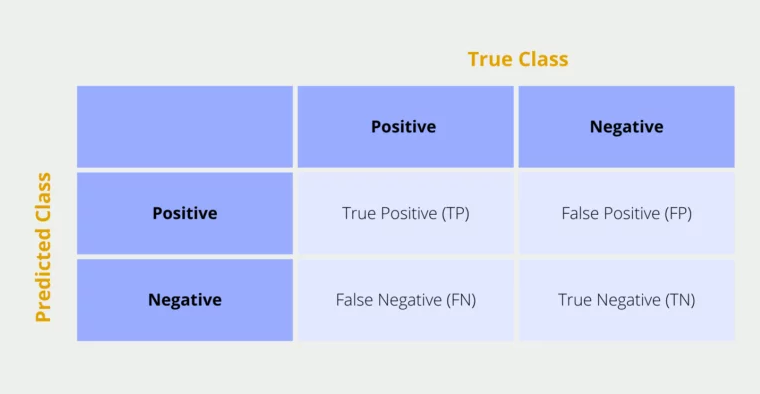
\includegraphics[width=8cm]{fig/confusion_matrix.png}
  \caption{Confusion Matrix \cite{confusion}.}%
  \label{fig:confusion-matrix}
\end{figure}

\textbf{Recall} \\ \\
Recall measures the fraction of positive instances that are correctly classified.

\begin{equation}
	R = \frac{TP}{TP + FN}
\end{equation}

\textbf{Precision} \\ \\
Precision measures the correctly classified positive instances in relation to the overall number of positively predicted instances

\begin{equation}
	P = \frac{TP}{TP + FP}
\end{equation}

\textbf{F1-Score} \\ \\
The F1 score is the harmonic mean between recall and precision.

\begin{equation}
	\text{F1} = \frac{2 \cdot P \cdot R}{P + R}
\end{equation}

To evaluate our models, we will only use the F1-Score to give a good comparison to similar works like the Validity and Novelty Prediction Shared Task \cite{argsvalnov2022}.

\section{Datasets}

We will primarily use two datasets. One for validity classification and one for stance classification. In this chapter will introduce both of them, describe our preprocessing and also mention additional data we are going to use besides these datasets.

\subsection{Validity Dataset}

The dataset for validity classification is taken from the shared task on predicting validity and novelty of arguments \cite{argsvalidnovel2022}. After discarding columns that are irrelevant for our work, each sample consists of the following columns:
\begin{enumerate}
	\item[\textbullet] Topic: Title of the debate
	\item[\textbullet] Premise: Some sentence about the topic
	\item[\textbullet] Conclusion: Conclusion of the premise
	\item[\textbullet] Validity
	\begin{enumerate}
		\item[-] Label 1: Conclusion is valid.
		\item[-] Label 0: Conclusion is defeasibly valid (This label is not contained in the test set. Hence we discard it completely).
		\item[-] Label -1: Conclusion is invalid.
	\end{enumerate}
\end{enumerate}
The data is already split in train, dev and test datasets, with a ratio of roughly $0.5$, $0.15$, $0.35$ and the dev and test set do not share the same topics with the train set. In the training set, about $53\%$ of the data has the validity label 1 and in both dev and test set about $60\%$.

\subsection{Stance Dataset}

The dataset for stance classification is taken from the the IBM project debater datasets \cite{stancedata, ibm}. Again, we discard unused columns, resulting in the following columns:
\begin{enumerate}
	\item[\textbullet] Topic: A statement about an arbitrary topic.
	\item[\textbullet] Argument: Argument regarding the topic.
	\item[\textbullet] Stance: Stance of the argument towards the topic.
	\begin{enumerate}
		\item[-] Label 1: Positive stance.
		\item[-] Label -1: Negative stance.
	\end{enumerate}
\end{enumerate}
The data is split with a ratio of about $0.7$, $0.2$, $0.1$ in train, dev and test data. Both labels roughly have a $50\%$ probability of occurrence.

\subsection{Additional Data}

Since not a lot of samples from both datasets, do not include conclusions or arguments that start with linking word, we decided to pretrain our models on artificially created data that explicitly uses linking words. To generate this data, we used ChatGPT \cite{chatgpt}, using prompts of the form
\begin{center}
	\textit{give me ten arguments consisting of multiple sentences and a conclusion that is indicated with <linking word>}.
\end{center}

Where we replace <linking word> with each of the linking words, we decided to use. 

\subsection{Preprocessing}

Besides the standard BERT preprocessing which consists of splitting strings in sub-word tokens and converting these strings to ids \cite{bertprepro}, we decided to combine all the different columns of the datasets that contain text (e.g. Premise, Conclusion) into one column in the following way:
\begin{enumerate}
	\item Add markers to the start of each column: <\_t> for the topic column, <\_p> for the premise column, <\_c> for the conclusion or argument column.
	\item Concatenate the columns to one text column.
	\item Add punctuation between the columns.
\end{enumerate}

After preprocessing, one data point looks like this:
\begin{center}
\raggedright
"<\_t> TV viewing is harmful to children. <\_p> The popularity of TV watching is among the reasons of this phenomenon. Violence, aggression, crimes and wars are broadcast through the daily news as well as in movies, showing dark pictures that encourage psychological tension, pessimism and negative emotions. <\_c> Depression is a well-known psychological problem of modern society that is partly caused by TV watching."
\end{center}

\section{Algorithms}
In this chapter, we will present all used algorithms and models for both classification tasks.

\subsection{Baseline}
To compare the performance of our models, we use a simple BERT classifier \cite{bert} as baseline. We use the training procedure and model from huggingface \cite{berttraining} with the standard parameters proposed in the original BERT paper \cite{bert}.

\subsection{Our approach}

This section is about describing all the necessary steps for our approach and explaining why we thought these steps are sensible. The approach consists of the following steps, as shown in figure \ref{fig:model-architecture1}:

\begin{enumerate}
	\item Generate embeddings for each data point based on probabilities for linking words.
	\item Concatenate these embeddings with BERT embeddings.
	\item Classify the combined embeddings.
\end{enumerate}

\begin{figure}[h]
  \centering
  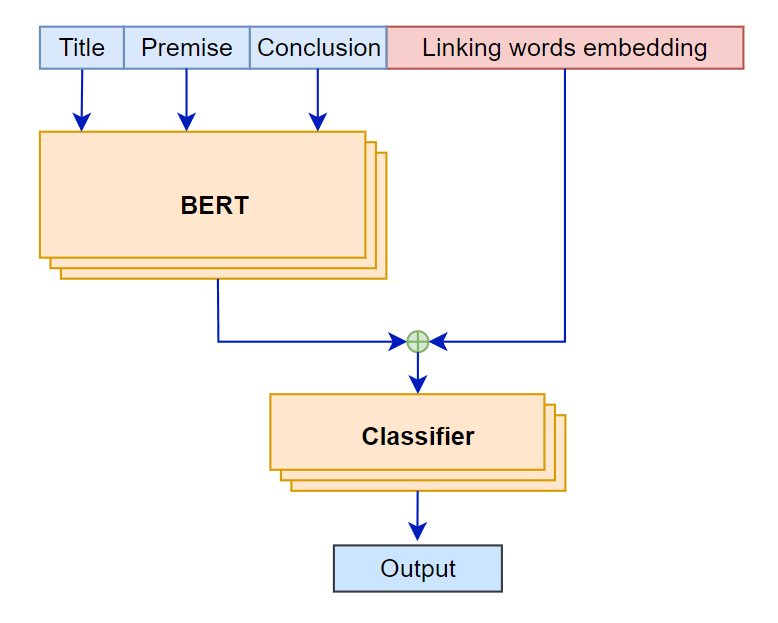
\includegraphics[scale=0.8]{fig/model_diag1.png}
  \caption{Model Architecture for validity classification: BERT transforms the text to embeddings. These are concatenated with linking words embeddings and then classified.}%
  \label{fig:model-architecture1}
\end{figure}

The main idea of our algorithm is taken from natural language. Often times in natural language, conclusions or arguments are indicated using linking words like \dq therefore\dq or \dq thus\dq. We want to use this fact to improve the performance of our baseline model by combining embeddings generated by BERT with custom embeddings depending on these linking words. In the next section, we will discuss exactly how these custom embeddings are created.

\subsubsection{Linking words embeddings}
To generate our custom embeddings, we will use BERT for masked language modeling. We start by training a BERT model for masked language modeling \cite{bertmask} on our data. For this, we just take one data point as one input sequence without [SEP] tokens in between the sentences, regardless of the number of sentences. After training, we add a [MASK] token to the start of every conclusion/argument. This extended data is then used to let BERT predict words for the [MASK] token. BERT yields a list of all the words in the vocabulary and their corresponding probabilities to be at the position of that [MASK] token. Now we define a set of linking words $\mathcal{L}$ and extract the probabilities for each linking word of $\mathcal{L}$ from the list of probabilities from BERT. This gives us a vector $E$ of probabilities with length $|\mathcal{L}|$ for each data point. This set of vectors is the final linking words embedding. \\

When looking at these embeddings however, we can see one problem. The probabilities tend to be very low and therefore the differences between probabilities are very low. One possible explanation could be that the data BERT was originally trained on, does not contain a lot of our chosen linking words and hence gives them a relatively low probability compared to more common words which would also fit in this position. One way to increase these values is to compare them to another value and use the relative difference as new value. We decided to do that in the following way: \\
Given a word vector embedding $E$, we build a matrix $M_E$ by applying the outer product between $E$ and $\frac{1}{E}$: $M_E = E \otimes \frac{1}{E} = E \cdot (\frac{1}{E})^T$.
Afterwards, we remove the diagonal entries of this matrix since these are all $1$ to get $M_E'$ and transform this matrix row wise into a vector: $E_{matrix} = vec(M_E')$ (see figure \ref{fig:transform1}). This new embedding has length $|\mathcal{L}| \cdot (|\mathcal{L}|-1)$.

\begin{figure}[h]
	\centering
	$$ M_E = \begin{pmatrix}
		e_1\\
        e_2\\
        \vdots\\
        e_{|\mathcal{L}|}
     \end{pmatrix}
     \cdot
     \begin{pmatrix}
     	\frac{1}{e_1} & \frac{1}{e_2} & \cdots & \frac{1}{e_{|\mathcal{L}|}}
     \end{pmatrix} = 
	 \begin{pmatrix}
		\frac{e_1}{e_1} & \frac{e_1}{e_2} & \cdots & \frac{e_1}{e_{|\mathcal{L}|}}\\
        \frac{e_2}{e_1} & \frac{e_2}{e_2} & \cdots & \frac{e_2}{e_{|\mathcal{L}|}}\\
        \vdots & \vdots & \ddots & \vdots\\
        \frac{e_{|\mathcal{L}|}}{e_1} & \frac{e_{|\mathcal{L}|}}{e_2} & \cdots & \frac{e_{|\mathcal{L}|}}{e_{|\mathcal{L}|}}
     \end{pmatrix}     
     $$
     
     $$
	 M_E' =   
	 \begin{pmatrix}
		\frac{e_1}{e_2} & \frac{e_1}{e_3} & \cdots & \frac{e_1}{e_{|\mathcal{L}|}}\\
        \frac{e_2}{e_1} & \frac{e_2}{e_3} & \cdots & \frac{e_2}{e_{|\mathcal{L}|}}\\
        \vdots & \vdots & \ddots & \vdots\\
        \frac{e_{|\mathcal{L}|}}{e_1} & \frac{e_{|\mathcal{L}|}}{e_2} & \cdots & \frac{e_{|\mathcal{L}|}}{e_{|\mathcal{L}|-1}}
     \end{pmatrix}  
     $$
     
     $$
     E_{matrix} = vec(M_E') = 
     \begin{pmatrix}
     	\frac{e_1}{e_2}  \frac{e_1}{e_3}  \cdots  \frac{e_1}{e_{|\mathcal{L}|}}  \frac{e_2}{e_1}  \frac{e_2}{e_3}  \cdots \frac{e_2}{e_{|\mathcal{L}|}}  \cdots  \frac{e_{|\mathcal{L}|}}{e_1} \frac{e_{|\mathcal{L}|}}{e_2}  \cdots  \frac{e_{|\mathcal{L}|}}{e_{|\mathcal{L}|-1}}
     \end{pmatrix}^T
     $$
     
	\caption{Transformation from $E$ to $E_{matrix}$}%
	\label{fig:transform1}
\end{figure}

In the following chapters, we will always use $E$ as embedding to describe the other steps. They work analogously for $E_{matrix}$.

\subsubsection{BERT embeddings}
As described in chapter 2, BERT outputs a vector representation for each token in the sequence, including special tokens. To generate embeddings for the entire sequence, we have to somehow transform these vectors into one. \\
Given an input sequence of length $l$, including all special tokens, BERT produces an output representation of shape ($l$, $H$) where $H$ is the hidden dimension of BERT (in our case always $768$). We will use two different ways to generate an embedding of shape ($1$, $H$) which we can then use for classification. The first way is the standard way explained in chapter 2, proposed by Delvin et. al. \cite{bert}. It assumes that the first token in the sequence, namely the [CLS] token, can be used as an aggregate representation of the entire sequence an hence be a suitable embedding for it. The other way is taking the average of all the token vectors along the first dimension. Both ways yield the desired embedding vector of shape ($1$, $H$).

\subsubsection{Classifier}
We are using two different classifiers. The first one is a simple neural net. We use the same architecture as the one that is used in BertForSequenceClassification from the transformer package \cite{bertimpl}. It consists of one dropout layer and one linear layer, followed by a softmax layer and the loss function, as shown in figure \ref{fig:nn1}. In the case of using the concatenated embeddings, the linear layer transforms the input matrix from shape $(D, \, |E| + H)$ to shape ($D$, $2$) where $D$ is the number of data points in the dataset. 

\begin{figure}[h]
  \centering
  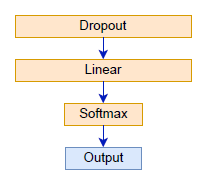
\includegraphics[scale=1]{fig/nn_1.png}
  \caption{Neural network classifier.}%
  \label{fig:nn1}
\end{figure}

For the second classifier, we will use a gradient-boosted tree, precisely LightGBM \cite{lgbm}.

\subsubsection{Feature selection}
Before passing the embedding vectors to the classifier, we apply feature selection to improve the performance of our model, by discarding features with low importance. This importance is calculated by the built-in method of LightGBM \cite{lgbmimportance}. We use different metrics to decide below which importance features are discarded, e.g. discarding all features whose importance is below the mean importance. We will present all of the metrics in the evaluation chapter.

\subsubsection{Summary}
Combining all steps, gives us the model shown in figure \ref{fig:model-architecture_full}. We will evaluate all the introduced techniques in different configurations. All the exact configurations will be explained in the evaluation chapter.

\begin{figure}[h]
  \centering
  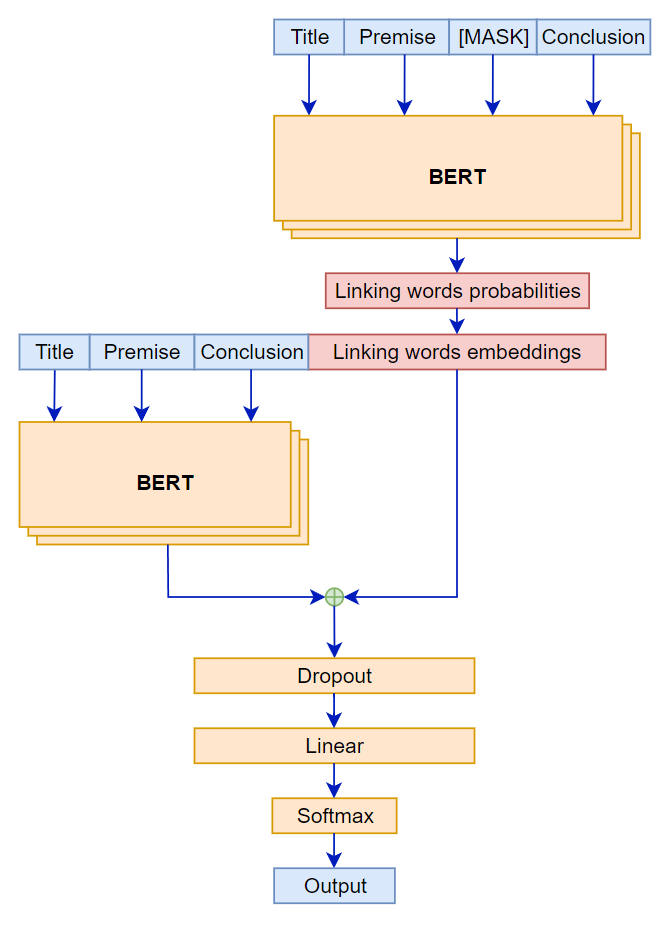
\includegraphics[scale=0.7]{fig/model_full.png}
  \caption{Complete Model Architecture for validity classification.}%
  \label{fig:model-architecture_full}
\end{figure}











%% Dieser Part kann auskommentiert werden, sollte kein Anhang nötig sein.
%% Der \appendix-Befehl leitet hierbei den Anhang ein.
 \appendix
 \section{Additional Linking Word Lists}

Our used $90$ linking words, taken from \cite{linking}. We only used phrased consisting of one word.

$L_3$ = [
		accordingly,
        consequently,
        hence,
        then,
        therefore,
        thus,
        absolutely,
        chiefly,
        clearly,
        definitely,
        especially,
        even,
        importantly,
        indeed,
        naturally,
        never,
        obviously,
        particularly,
        positively,
        surprisingly,
        truly,
        undoubtedly,
        additionally,
        also,
        and,
        besides,
        finally,
        first,
        further,
        furthermore,
        last,
        moreover,
        second,
        third,
        too,
        including,
        like,
        namely,
        specifically,
        alternatively,
        conversely,
        however,
        instead,
        nevertheless,
        nonetheless,
        nor,
        notwithstanding,
        rather,
        though,
        unlike,
        whereas,
        while,
        yet,
        alike,
        both,
        either,
        equal,
        equally,
        likewise,
        resembles,
        similarly,
        altogether,
        briefly,
        overall,
        ultimately,
        as,
        if,
        since,
        unless,
        when,
        whenever,
        lest,
        concerning,
        considering,
        regarding,
        reiterated,
        regularly,
        typically,
        mostly,
        normally,
        often,
        commonly,
        because,
        although,
        but,
        still,
        for,
        so,
        anyway,
        mainly
]

The $90$ most common English words according to \cite{mostcommon}.

$L_4$ = [the,
        be,
        to,
        of,
        and,
        a,
        in,
        that,
        have,
        I,
        it,
        for,
        not,
        on,
        with,
        he,
        as,
        you,
        do,
        at,
        this,
        but,
        his,
        by,
        from,
        they,
        we,
        say,
        her,
        she,
        or,
        an,
        will,
        my,
        one,
        all,
        would,
        there,
        their,
        what,
        so,
        up,
        out,
        if,
        about,
        who,
        get,
        which,
        go,
        me,
        when,
        make,
        can,
        like,
        time,
        no,
        just,
        him,
        know,
        take,
        person,
        into,
        year,
        your,
        good,
        some,
        could,
        them,
        see,
        other,
        than,
        then,
        now,
        look,
        only,
        come,
        its,
        over,
        think,
        also,
        back,
        after,
        use,
        two,
        how,
        our,
        work,
        first,
        well,
        way]

\section{Discarded Ideas}
We tried a vast number of ideas to improve the performance of our models but discarded a lot after evaluating them and getting subpar results. In this section, we are going to list a few of these ideas:

\begin{itemize}
	\item Calculating the perplexity of the model depending on the seen linking word at the beginning of a conclusion/argument 			  for each linking word. This was then used as the linking word embedding or extended the embedding.
	\item Using different classifiers like SVMs or a nearest neighbor classifier using cosine distance.
	\item Standardizing the embeddings to have mean $0$ and standard deviation $1$.
	\item Only using the linking word embeddings for classification instead of concatenating them with the LM embeddings.
\end{itemize} 

As already mentioned in the evaluation, we decided not to show the results of some ideas that still had good results, due to the fact that they were too similar to the presented results. Examples for that are additional pretraining, and using RoBERTa instead of BERT.

%%%%%%%%%%%%%%%%%%%%%%%%%%%%%%%%%%%%%%%%%%%%%%%%%%%%%%%%%%%%%%%%%%%%%%%%%%%%%%%%
%% (Ende) Der Inhalt der Arbeit                                               %%
%%%%%%%%%%%%%%%%%%%%%%%%%%%%%%%%%%%%%%%%%%%%%%%%%%%%%%%%%%%%%%%%%%%%%%%%%%%%%%%%


\backmatter

%% Listings of figures, tables, etc. Delete what is not needed.
\listoffigures\thispagestyle{headings}

\listoftables\thispagestyle{headings}

% Algorithms
\listofalgorithms\thispagestyle{headings}

% Code Listings
\lstlistoflistings\thispagestyle{headings}

\clearpage
\bibliography{references}
%% Depending on Language, use german alphadin or original alpha
\iflanguage{ngerman}{
  \bibliographystyle{alphadin}
}{
  \bibliographystyle{alpha}
}

\end{document}
